\vspace{-0.1in}
\section{Evaluation}
\label{sec:eval}
In this paper, we attempt to address performance concerns in the switchless architecture: how does the performance compare when running a workload like weather modeling or Apache's Hadoop~\cite{Apache:Hadoop}? To this end, we simulate a micro-benchmark with parameters that approximate real workloads on two switchless topologies (torus and cube), and two traditional topologies (fat-tree and hierarchical). As alluded to in Section~\ref{sec:arch}, we do not expect switchless to have higher performance than a fat-tree on all applications. Yet, with the massive force of low-cost attached to switchless, we would hope that any performance degradation would be acceptable.

%We also ran a few more benchmarks such as a bandwidth stress test to see the effect of increasing data transfer rate, as well as the efficiency of UDP vs TCP.
We also ran other simulations to compare the overhead of UDP versus TCP in the data center setting, as well as IP routing versus dimension-ordered routing.

\subsection {Methodology}
For performance evaluation, we use the ns-3 simulator\cite{Ns3:Online}, an open-source discrete-event network simulator developed by the networking research community. We modified a significant portion of the simulator for our purposes. These modifications include adding a dimension ordered routing protocol, creating various network topologies for both switchless and conventional architectures, and constructing a highly configurable synthetic micro-benchmark.  Due to time constraints, we did not modify ns-3 to implement wormhole routing and do not make any claims about it in our evaluation.  The ns-3 simulator, augmented with our modifications, models all five OSI stack layers.

As it is hard to define a small representative application for the data center, we used a synthetic micro-benchmark that can be configured to model various application communication pattern. For example, this micro-benchmark can be configured to generate simple all-to-all style communication traffic with certain intensity. On the other hand, it can also be configured to generate sporadic communications between two random nodes. Note that there are many other possible configurations which create different communication patterns for modeling application communication patterns.

% benchmark configurations (common)
The default configurations for all simulations are detailed in Table~\ref{tab:configurations}, unless noted specifically.  All switchless topologies (torus and cube) use dimension ordered routing, while all traditional topologies (conventional hierarchy and fat-tree) use IP routing, unless otherwise specified.
% # host: 512
% Ethernet links: 1Gbps
% hierarchical: 1 core, balanced fan-outs (agg / edge == edge / host)
% link/switching latency is 500ns for all topologies!!!!!!!!!!! (might be wrong)
% cube z-dimension limit is 40
% all topologies are running on UDP
% switchless are using dimension ordered routing
% 4KB packet length

\subsection {Results}
% Results -- 
% (1) Impact of topology change on performance
% (2) Impact of routing change on performance
% (3) Application Sensitivity (Different application configurations)
% (4) Scalability (host count change)

The following sections present simulation results for different communication patterns and protocols.


\subsubsection{All-to-All Communication}\label{sec:all-to-all-communication}
\newcommand{\nbody}{N-Body}
In all-to-all communication, all nodes communicate to all other nodes.  This type of communication pattern is representative of applications such as \nbody~simulations and other data center applications in which nodes must communicate to all other nodes. Figure~\ref{fig:nbody_packetdelay} shows the packet delay distribution of all packets sent in one computation round of an all-to-all simulation for all topologies and network stacks; Figure~\ref{fig:nbody_latency} shows the longest packet delay--the global communication latency of a computation round--compared.

\captionsetup[subfloat]{captionskip=-0.003in}
\begin{figure}
    \centering
    \subfloat[Packet Delay Distribution]
    {
        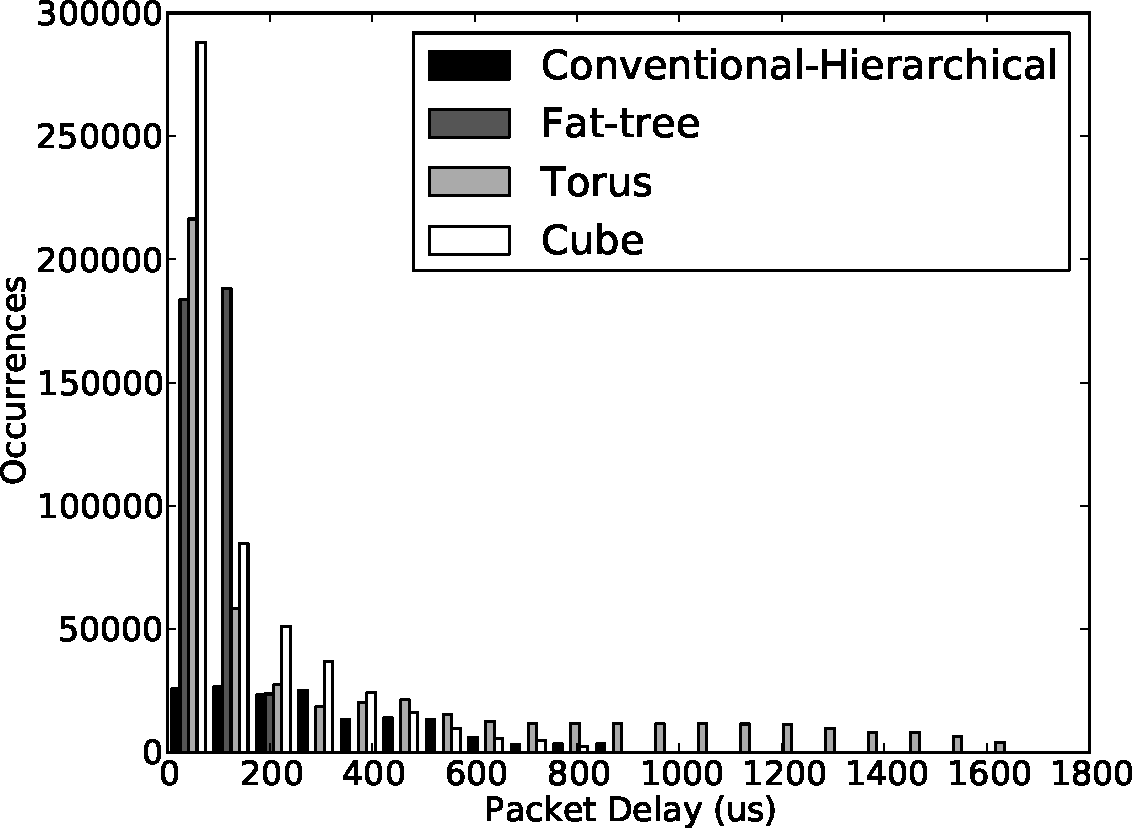
\includegraphics[width=0.25\textwidth]{nbody_delay}
        \label{fig:nbody_packetdelay}
    }
    \\
    \vspace{-0.1in}
    \subfloat[Longest Delay]
    {
        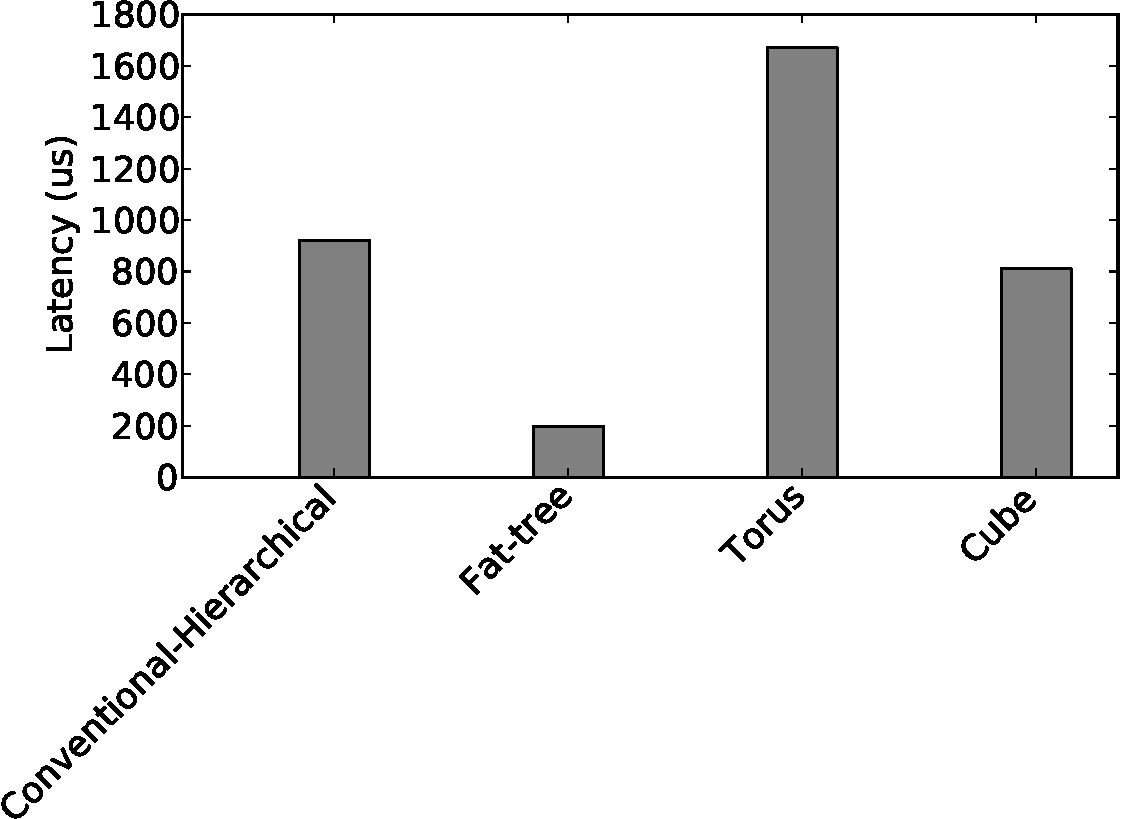
\includegraphics[width=0.25\textwidth,trim={0 3.1cm 0 0},clip]{nbody_latency.pdf}
        \label{fig:nbody_latency}
    }
    \vspace{-0.07in}
    \caption{All-to-All Simulation Results}
    \label{fig:common_topos}
\end{figure}

While switchless topologies have higher occurrences of short packet delay (nodes close together), there are also a small number of packets with long delays (nodes far away) that limit the global computation throughput of all-to-all computation. As shown in Figure~\ref{fig:nbody_latency}, fat-tree is about four times faster than cube and conventional hierarchy, and as much as seven times faster than the torus topology.

On the other hand, it does not necessarily mean that simulation under fat-tree is four times faster than cube: the computational time is needed to compute overall performance.  In addition, all-to-all communication is not a communication pattern that matches well with switchless topologies, as lots of congestion will be created when every node sends to every other node and the maximum hop count is higher.  Fat-tree topologies match better with this type of communication pattern.
% perhaps we need a plot here, comparing different topologies' time in y axis with computational time in the x axis.

\subsubsection{Random N to random M}
In Figure~\ref{fig:25_packetdelay} and Figure~\ref{fig:25_latency}, we have the cube topology performs better than other topologies.

\captionsetup[subfloat]{captionskip=-0.003in}
\begin{figure}
    \centering
    \subfloat[Packet Delay Distribution]
    {
        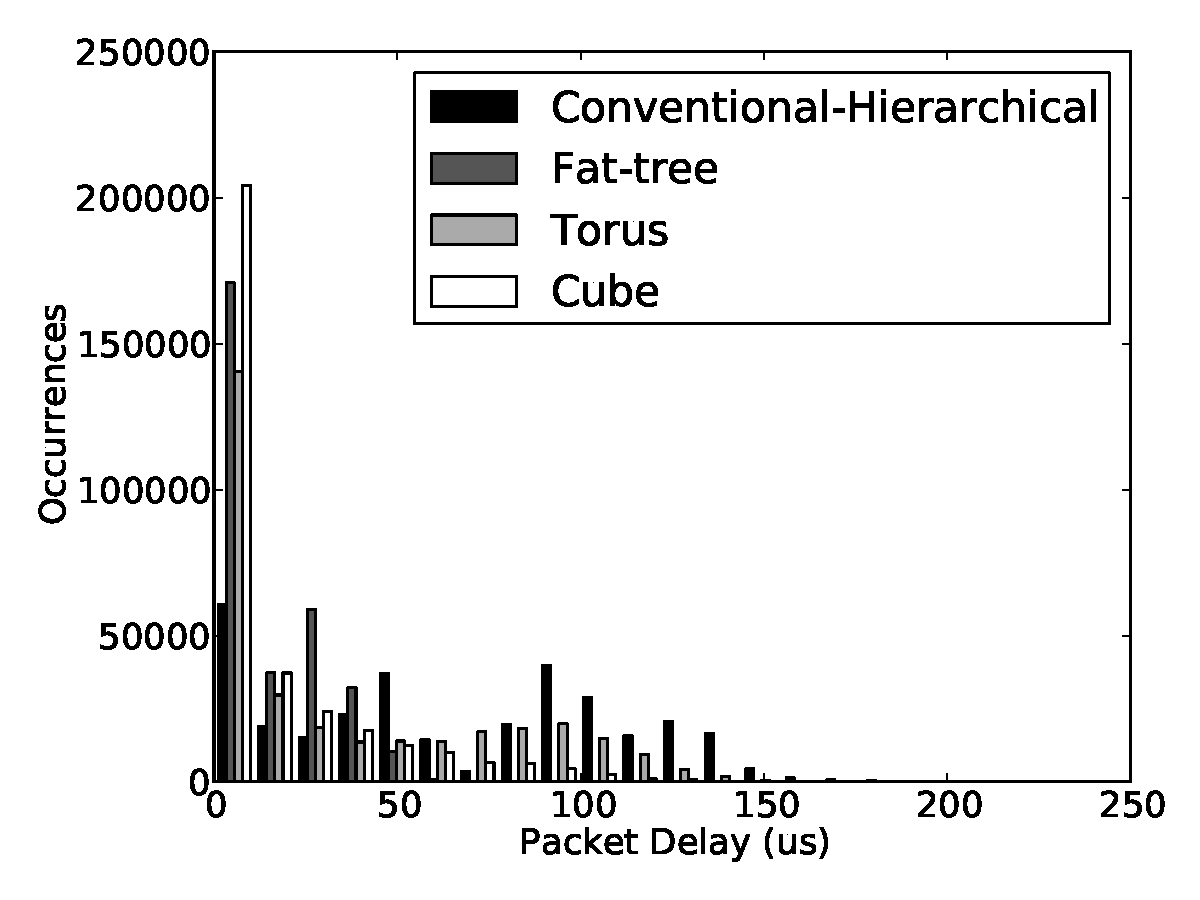
\includegraphics[width=0.25\textwidth]{25_delay}
        \label{fig:25_packetdelay}
    }
    \\
    \vspace{-0.1in}
    \subfloat[Longest Delay]
    {
        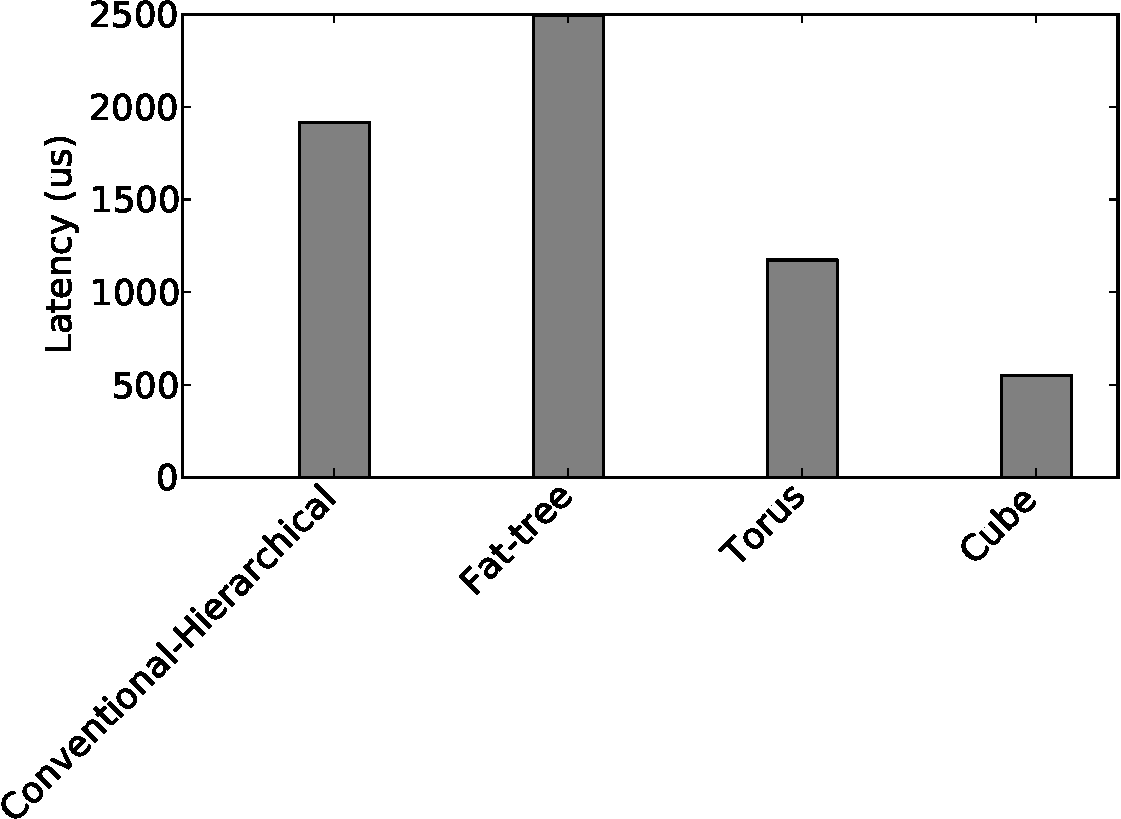
\includegraphics[width=0.25\textwidth,trim={0 3.75cm 0 0},clip]{25_latency.pdf}
        \label{fig:25_latency}
    }
    \vspace{-0.07in}
    \caption{RNRM Simulation Results}
    \vspace{-0.1in}
\end{figure}


%\subsubsection{TCP versus UDP}
%Data center operators usually run TCP as the level 4 networking stack~\cite{Regnier:2004:TCPODCS,Alizadeh:2010:DCT,Kandula:2009:NDC}. However, TCP has more overhead compared with UDP, and TCP guarantees are not necessary in data centers where dropped packet are rare. As we utilize a full network stack simulator for our study, we implement our topologies with both TCP and UDP and run a simulation exercise to see how the overheads compare.

%What we found was that, at least for our simulation set up, TCP has about the same performance as UDP, but packet drops are more frequent, leading to completion time timing out.


\subsubsection{Dimension Ordered Routing versus IP Routing}
As mentioned, for switchless topologies, we had two implementations: one with TCP/IP routing, and the other one with dimension-ordered routing commonly used in networks on chip. In our simulation, as shown in Figure~\ref{fig:dim_ordered}, we found that dimension ordered routing is slower than IP routing. One possible reason for this is that dimension-ordered protocol restricts the possible data paths that packet can traverse, thereby introducing bandwidth contention that otherwise might not exist in traditional IP routing.  In addition, ns-3 does not model the time to make routing decisions or the latency to switches/routers.  Thus, we are unable to model the faster dimension ordered routing decisions and integrating the switch with the processor.  Further, due to time constraints, we were not able to model the benefits from using wormhole routing with dimension ordered routing.  We believe if we had, we would have seen large performance improvements over IP routing.

\captionsetup[subfloat]{captionskip=-0.003in}
\begin{figure}
    \centering
    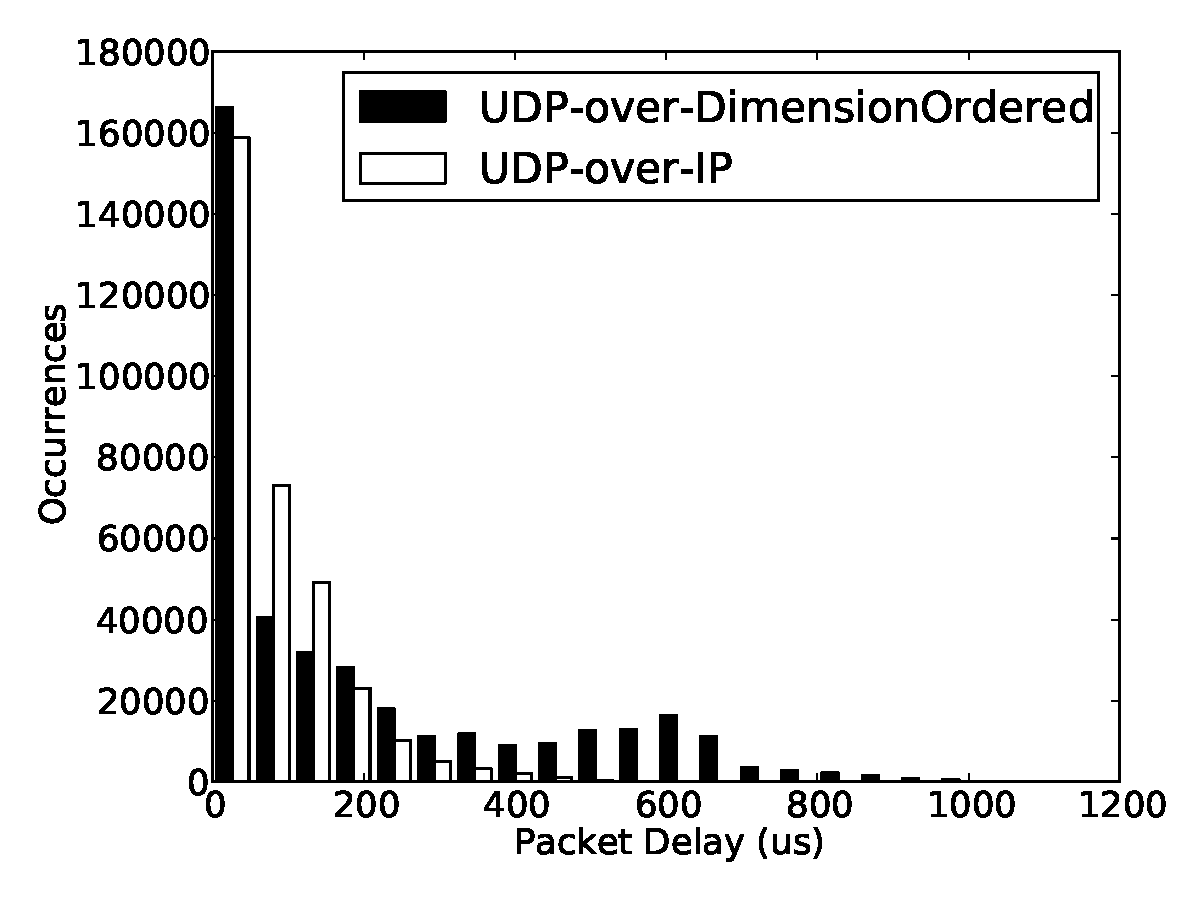
\includegraphics[width=0.22\textwidth]{dimension_ordered_udp}
    \vspace{-0.1in}
    \caption{Packet Delay Distribution of a Torus Network Running UDP Over IP and UDP Over Dimension Ordered.}
    \label{fig:dim_ordered}
    \vspace{-0.1in}
\end{figure}

